\section{Grafy automatów}

\subsection{Słówko o automatach}

Automaty Moore'a i Mealy tworzone są na przerzutnikach, więc posiadają pamięć. Każdy automat posiada swój stan początkowy i na podstawie ciągu wprowadzonych danych w odpowiednich cyklach zegarowych (zegar może być sterowany ręcznie). Automat ma dać odpowiedni sygnał wejściowy w zależności od wprowadzonych danych. Automaty to układy cyfrowe realizujące zadane sekwencje (detekcję ciągu, odczytanie słów itp.). Rozróżniamy na naszych zajęciach dwa rodzaje automatów: Moore'a i Mealy. Różnica na dobrą sprawę polega tylko na tym, że w tych pierwszych na wyrysowanym grafie wyjścia znajdują się na stanach, a w drugim - na przejściach. Graf tworzymy prosto z treści zadania. W automatach Moore'a zazwyczaj ostatni stan to jest ten, w którym dana sekwencja jest akceptowana, więc nasze wyjście to $y_1$, pozostałe stany mają $y_0$. Automat Mealy ma wyjścia na przejściach, toteż najczęściej stanów będzie mniej o 1. Z racji podanej wcześniej cechy, logiczna jedynka pojawi się na wyjściu od razu po wprowadzeniu danych, przed podaniem sygnału na wejście zegarowe przerzutników. Uniknąć tego można dokładając tuż przed wyjściem (diodą, odbiornikiem) kolejny przerzutnik (typu D) z podpiętym wejściem CLK i RESET. Wtedy, mimo iż układ został zbudowany na zasadach automatu Mealy, działa jak automat Moore'a.

\subsection{Treść zadania}

Automat będący detektorem sekwencji "0111"

\subsection{Graf automatu moore'a}

\begin{figure}[h!]
    \centering
    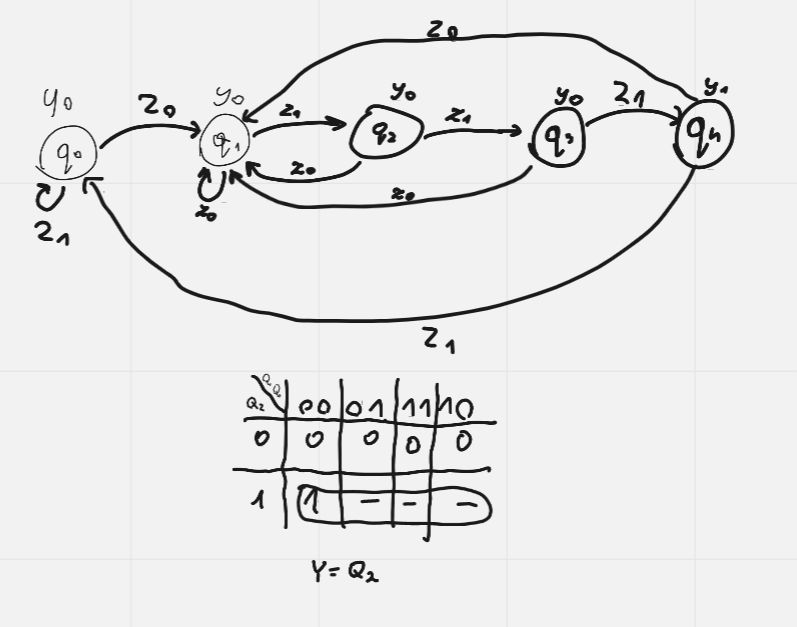
\includegraphics[width=.55\textwidth]{images/graph/g_moore.png}
    \caption{treść zadania}
    \label{fig:my_label}
\end{figure}

\newpage

\subsection{Graf automatu mealy'ego}

\begin{figure}[h!]
    \centering
    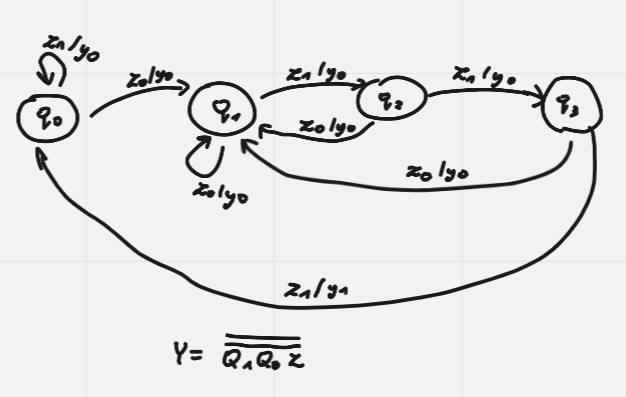
\includegraphics[width=.55\textwidth]{images/graph/g_mealy.png}
    \caption{treść zadania}
    \label{fig:my_label}
\end{figure}